% \textbf{\textit{What processes shape genetic variation both temporally and
%         spatially, partition evolutionary lineages, and generate and maintain
%         biodiversity?}} \\
\textbf{\textit{What processes control the generation and assembly of
        biodiversity?}}
This question is the primary motivation of my research program.
To elucidate answers, I use patterns of genetic variation within and among
species to identify independent evolutionary lineages (i.e., species) and infer
their demographic histories and relationships, testing for patterns predicted
by current ecological factors and historical events.
I use a broad suite of methods in this endeavor, including
% collection-based fieldwork,
fieldwork,
next-generation sequencing (NGS),
developing statistical procedures for inferring evolutionary
history from NGS datasets,
implementing such methods in software packages,
and ultimately applying these novel computational tools to genomic data to test
hypotheses about diversification.
% I take an integrative approach to answering open-ended questions about
% biodiversity, which requires critical thinking and creativity.
% As a result, it is imperative that I involve students with diverse
% backgrounds and interests, who can bring unique perspectives to the
% challenges in my lab.
Given the integrative nature of my research program, I seek to recruit students
with diverse backgrounds and interests.
The questions I am passionate about exploring are open-ended and require
critical thinking and creativity.
As a result, it is imperative that I involve students and collaborators with
diverse backgrounds and perspectives to bring together unique insights.

\subsection*{Previous Research}
%%%%%%%%%%%%%%%%%%%%%
% \subsection*{Diversification of Crocodiles}
% Traditionally, crocodiles (\emph{Crocodylus}) have been stereotyped as an
% ancient group of ``living fossils'' that originated in Africa prior to the
% fragmentation of Pangea; their diversity and circumtropical distribution was
% attributed to vicariance via continental drift.
% However, early molecular data and subsequent reassessment of paleontological
% data suggested the genus could be younger than previously believed.
% Recently, I collected a large multi-locus dataset of all extant crocodylian
% species and used novel statistical phylogenetic methods to infer the temporal
% and biogeographical origin of \emph{Crocodylus}.
% My results overturned traditional views of crocodiles as ``living-fossils''
% from Africa, revealing a recent and dynamic evolutionary history
% \footfullcite{Oaks2011}.
% My results strongly support that all extant crocodiles shared a common ancestor
% from the tropics of the Indo-Pacific, approximately 14--8 million years ago
% (mya), rejecting an ancient vicariant explanation of their biogeography in
% favor of a recent, dispersal-mediated model involving multiple transoceanic
% dispersals.
% It was not until after the mid-Miocene climatic optimum, when the global
% climate was cooling and fellow crocodylian lineages were suffering massive
% extinctions, that \emph{Crocodylus} radiated and dispersed around the globe.
% This finding suggests it was not only global cooling driving the extinction of
% other crocodylians, as previously believed, but also most likely competition
% with the rapidly radiating \emph{Crocodylus} lineage.
% %My results also revealed more species diversity within the \emph{Crocodylus}
% %than currently recognized.

% This study also introduced important methodological innovations.
% To accommodate the variation of substitution rates across DNA positions
% within and among genes, I used a novel approach of estimating the optimal model
% for partitioning the alignment into rate categories.
% The resulting model performed far better than traditional methods that
% partition the alignment based on \emph{a priori} expectations of rate variation
% \footfullcite{OaksInPrep}.
% This has important implications, because improved modeling of among-site rate
% variation will mitigate the underestimation of long branches and concomitant
% systematic error in phylogenetic estimates (e.g., long-branch attraction).
% Furthermore, the study was among the first to estimate a time-calibrated
% species tree using a multi-species coalescent model, and was the first to use a
% posterior sample of species trees to estimate ancestral-state reconstructions.
% % The species tree represents the evolutionary history of populations, rather
% % than the history of individual gene copies.
% Using a direct estimate of the species phylogeny, rather than the history of
% individual gene copies, is ideal when inferring the evolutionary patterns of
% species-level characters, like ancestral ranges.

\subsubsection*{Climate-driven diversification}
One question I am passionate about is whether Quaternary climatic oscillations
promoted diversification by fragmenting the distributions of species.
% One focus of my current research seeks to determine whether Quaternary climatic
% oscillations promoted diversification by fragmenting the distributions of
% species.
An ideal model system for addressing this question is the dynamic landscape of
Southeast Asia.
The Southeast Asian mainland and 26,000+ islands experienced dramatic cyclical
shifts in the extent of the terrestrial landscape during glacial cycles.
Many groups of islands in this region coalesced during glacial periods when sea
levels were lower than today; these islands were repeatedly fragmented during
interglacial rises in sea level.

% \begin{wrapfigure}{r}{0.44\textwidth}
%   \vspace{-1.5em}
%   \begin{center}
%       \fbox{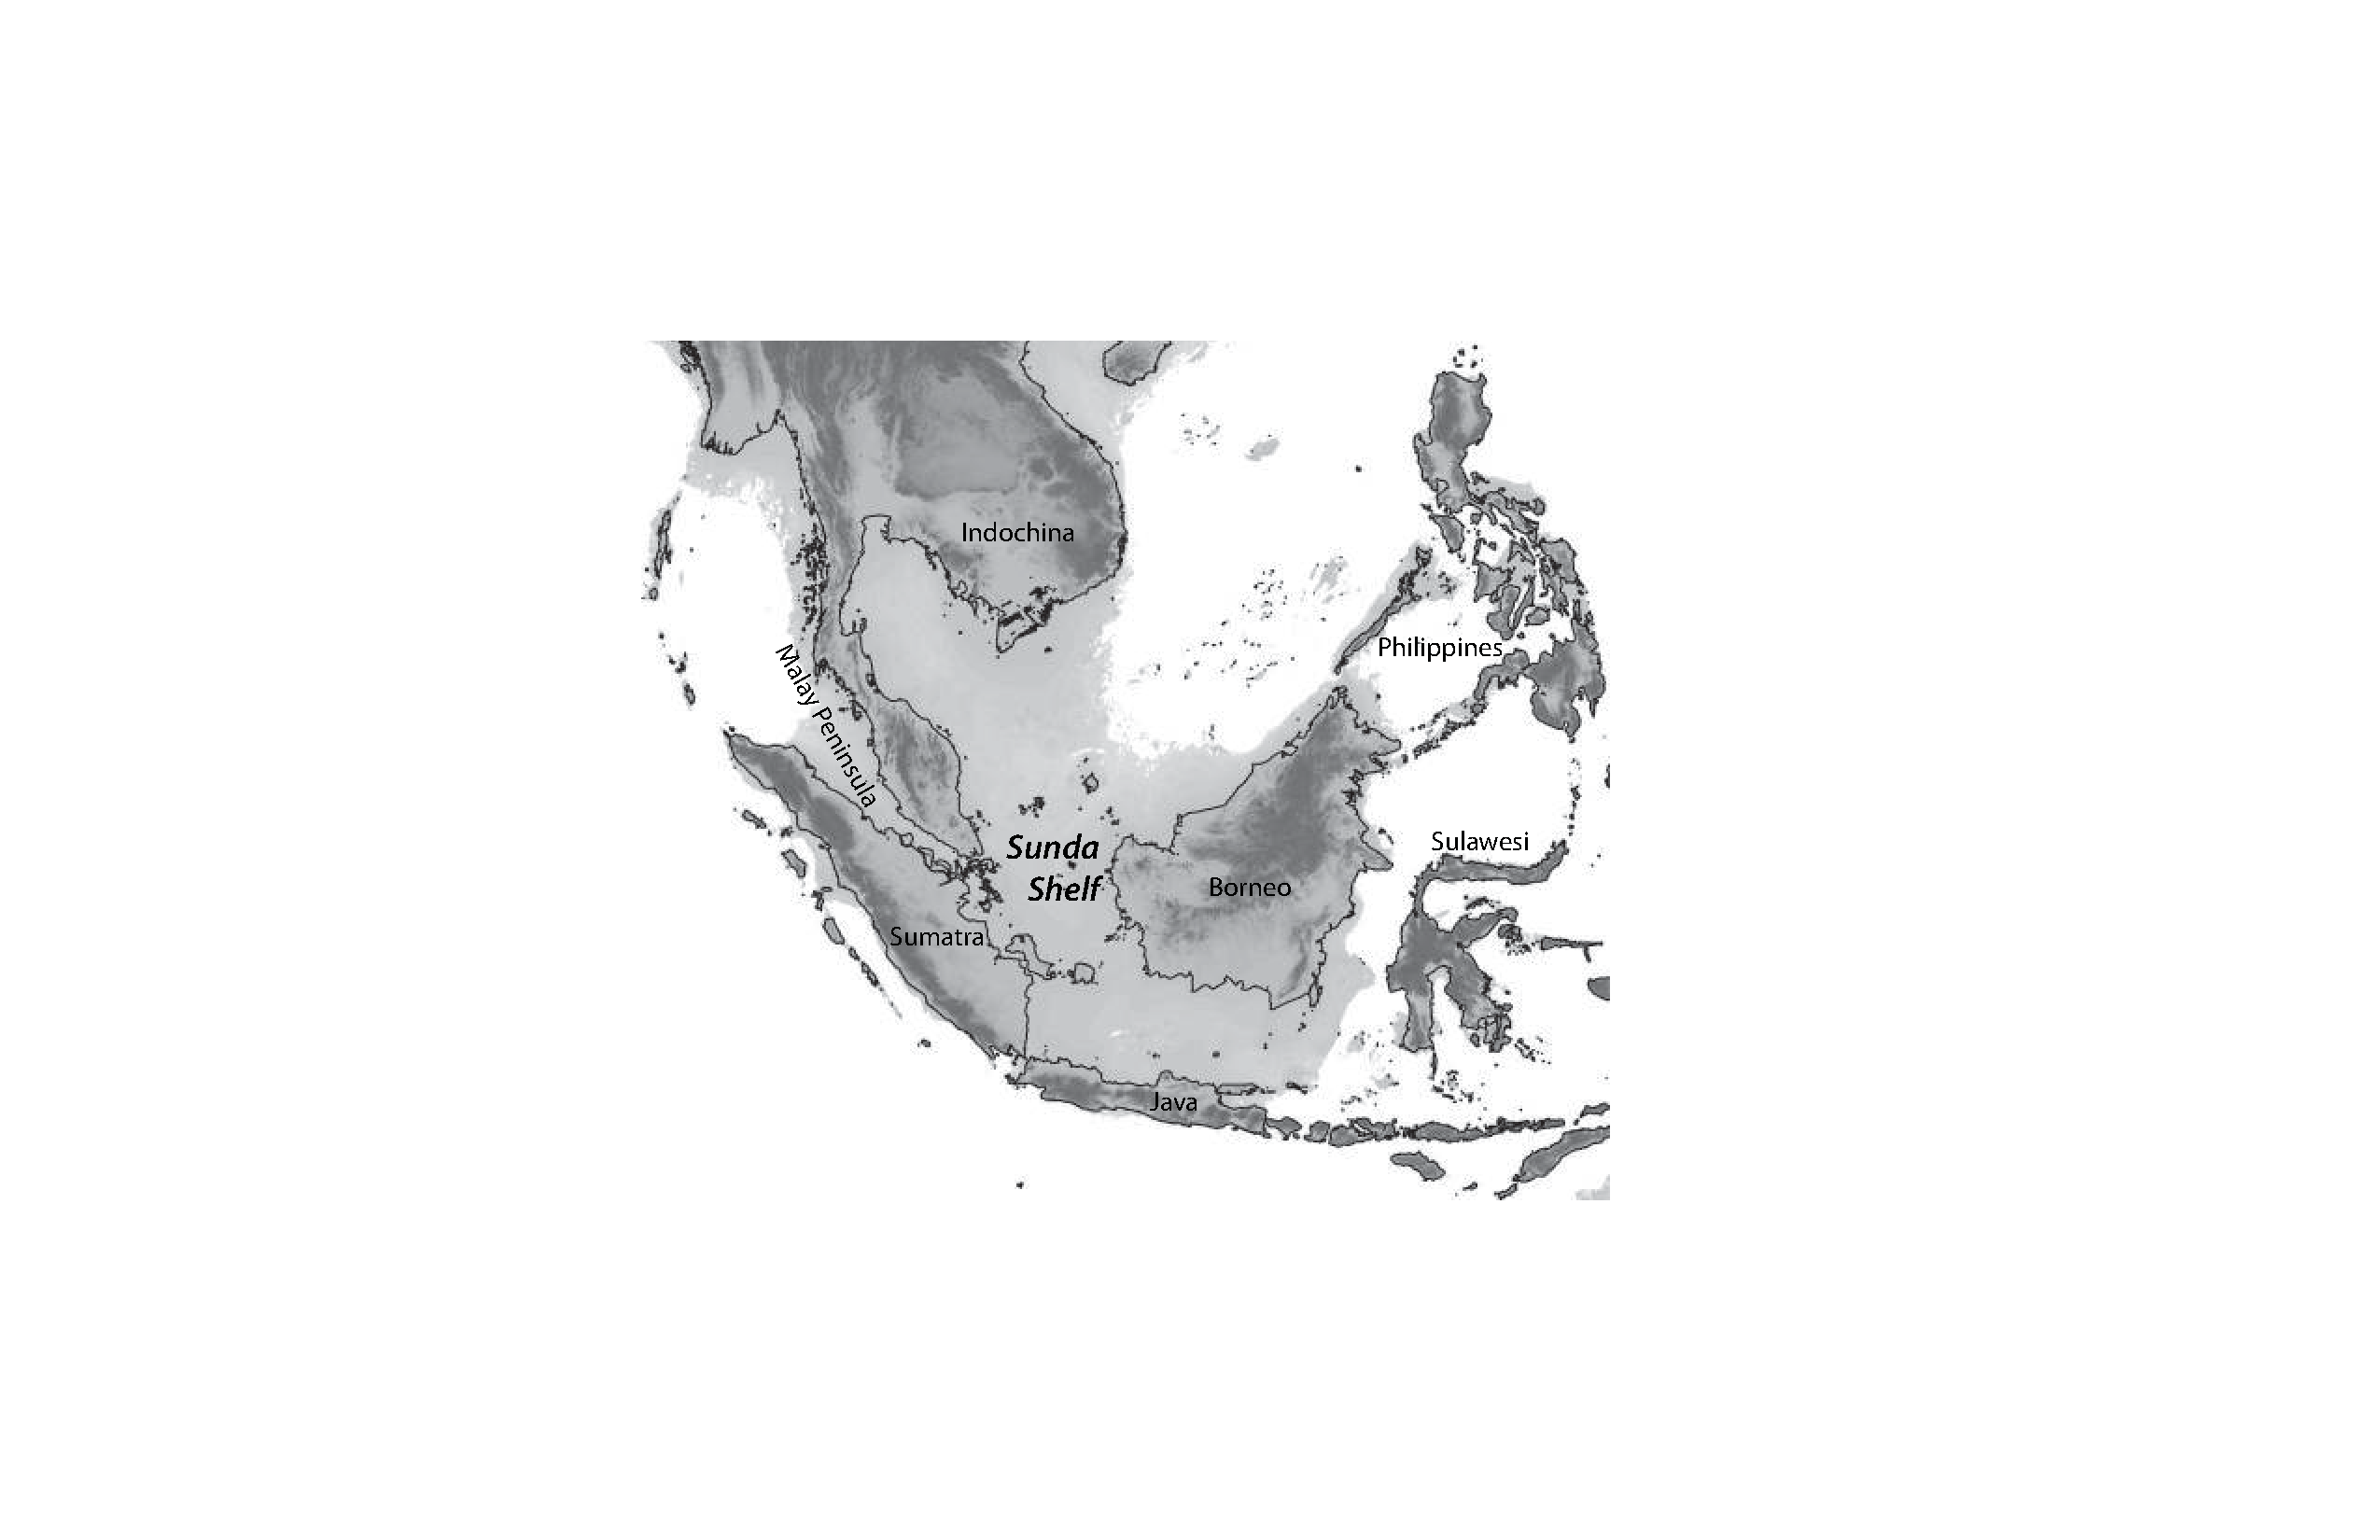
\includegraphics[width=0.43\textwidth]{sunda_shelf_very_small.pdf}}
%   \end{center}
%   \vspace{-0.2em}
%   \caption{Map of Southeast Asia with land extent (depicted in grey) during
%   glacial lowstands estimated using 120m bathymetry (data from
%   \href{http://ngdc.noaa.gov/mgg/global/global.html}{ETOPO1}).}
%   \label{map}
%   \vspace{-1.1em}
% \end{wrapfigure}

% To test whether the repeated fragmentation of island complexes
% promoted diversification, collaborators and I have been studying the
% evolutionary history of two genera of geckos (\emph{Cyrtodactylus} and
% \emph{Gekko}) that are co-distributed across most of the islands of the
% Philippines\footnote{\label{Siler10}\shortfullcite{Siler2010}}\super{,}\footnote{\label{Siler12}\shortfullcite{Siler2012}}.
% We found that populations within island complexes did explain a significant
% proportion of the genetic diversity, but were not monophyletic, and there was
% no obvious pattern of diversification associated with Pleistocene glacial
% cycles.
% We revealed complex histories for both genera that contradict many of the
% traditional areas of endemism predicted by island connectivity during glacial
% periods.
% Interestingly, for \emph{Gekko}, we found evidence that the genus colonized the
% Philippines by ``rafting'' on the Palawan Microcontinental Islands that rifted
% away from Mainland Asia and drifted toward the rest of the Philippine
% Archipelago.

To test whether glacial cycles promoted diversification,
collaborators and I used a broadly comparative approach\cref{Oaks12}.
We accumulated genetic data from island populations of 22 distantly related
taxa, representing five orders of terrestrial vertebrates.
For each taxon, we sampled genetic data from two populations currently on
separate Philippine Islands that were previously connected during glacial
periods.
If repeated bouts of island connectivity and isolation promoted
diversification, the temporal distribution of divergences across the 22
inter-island pairs of populations should be temporally clustered and correspond
to interglacial rises in sea level that fragmented the islands.
To test this prediction, we employed a popular Bayesian method,
msBayes, to estimate the probabilities of models in which multiple sets of taxa
diverged at the same time.
We found very strong support
% (posterior probability of 0.982)
for a single, recent, simultaneous divergence event shared by all 22 taxa.

Suspicious of such strong support given the richness and stochasticity of the
candidate models,
I used computer simulations to assess the ability of the msBayes method to
detect random variation in divergence times.
The results of the simulations revealed that the method will often strongly
support highly clustered models of divergence even when the taxa being compared
diverged randomly over millions of generations.
Thus, our results from the empirical Philippines data were likely spurious.
% This finding is important, because msBayes is a popular method, and results of
% clustered divergence times across co-distributed taxa are often interpreted as
% evidence for a shared historical event.
% Our results demonstrate that the method can be biased toward such results, and
% the interpretation of a shared event is not warranted without simulation-based
% validation of the method's performance.

% Needed better method---did it
Rather than abandon the approach, I formulated the full evolutionary model
underlying the msBayes procedure and, using first 
principles of probability, identified theoretical reasons the method
would tend to spuriously infer simultaneous divergence across
taxa\footnote{\label{Oaks12}\shortfullcite{Oaks2012}}\super{,}\footnote{\label{Oaks14reply}\shortfullcite{Oaks2014reply}}.
Guided by these insights, I developed a new model that uses more flexible prior
probability distributions for many of the models' parameters, and a
nonparametric Dirichlet-process prior across all possible divergence models.
I implemented the new model in the software package dpp-msbayes, and developed
a much more efficient multi-processing interface for both dpp-msbayes and
msBayes.
Using analyses of simulated and empirical data, I found, as predicted by
theory, the new method was much more accurate and robust\cref{Oaks14dpp}.
Applying this new method to the comparative Philippines dataset, I found a
large amount of uncertainty about the number of divergence events shared across
the 22 taxa.
% ; there simply was not enough information in our data to
% discriminate among models of divergence.
While such uncertainty is more intuitive than what we found with the original
method, it was empirically unsatisfying.
Thus, my current work focuses on developing more powerful methods that can
leverage large, comparative NGS datasets for addressing questions about
diversification.


\subsection*{Current Research}
%%%%%%%%%%%%%%%%%%%%%
I am developing and implementing novel comparative methods, collecting genomic
datasets from biodiverse regions of the planet, and applying the former to the
latter to enable unprecedented power to understand historical processes of
diversification across regions characterized by high levels of species richness
and endemism.  Below I detail one such method, and three empirical systems that
have inspired its development.

% Full likelihood method
\subsubsection*{Implementing a full-likelihood Bayesian model of
    co-diversification}
Both msBayes and dpp-msbayes use approximate likelihoods and discard
information when reducing genetic data to a set of insufficient summary
statistics.
Thus, dpp-msbayes still struggles to discriminate among models of divergence at
recent evolutionary timescales \footnote{\label{Oaks14dpp}\shortfullcite{Oaks2014dpp}}.
Given that such a statistical tool is integral to the evolutionary questions
I seek to answer in my empirical research,
I am currently developing a method that employs a similar hierarchical model in
a full-likelihood Bayesian framework.
% I am utilizing recent developments that analytically integrate over gene trees
% for biallelic data\footnote{\label{Bryant12}\shortfullcite{Bryant2012}}.
% This will remove the gene trees from the numerical approximation machinery and
% allow efficient sampling of divergence models and population divergence times
% using full likelihoods and Markov chain Monte Carlo.
By analytically integrating over gene trees, the method will efficiently handle
NGS datasets.
By utilizing all of the information in the data, the method promises to be much
more powerful than its approximate-Bayesian counterparts, and will also be
applicable at deeper evolutionary timescales.
This new tool will allow evolutionary biologists to better leverage comparative
genomic data to assess the affects of regional and global biogeographical
processes on biodiversity.

% Apply new method to genomic data from Philippine geckonids
\subsubsection*{Diversification across oceanic and mainland Southeast Asia}
% (2) collecting genome-scale data from dense sampling of \emph{Cyrtodactylus}
% and \emph{Gekko} from across the Philippine Archipelago using next-generation
% sequencing technology.
In addition to developing a full-likelihood Bayesian framework for inferring
co-diversification, I have also collected genome-wide sequence data from nearly
300 individuals of two genera of geckos (\emph{Cyrtodactylus} and \emph{Gekko})
from across the Philippine Archipelago using NGS technology.
The combination of the new method and NGS data will allow us to better assess
the affect of sea-level fluctuations on diversification across oceanic islands
of Southeast Asia.

To complement to this work on oceanic islands, I am also working with an
international team of collaborators
(Drs.\ Cameron Siler,
Lee Grismer,
Norhayati Ahmad,
Shahrul Anuar Mohd Sah,
and
Anchalee Aowphol)
to better understand diversification in
mainland Southeast Asia.
We are collecting a large comparative dataset of reptiles and amphibians from
across much of the Sunda Shelf, and will apply the
methods I am developing to test long-standing hypotheses about the affect of
biogeographical transition zones on the diversification of Sunda Shelf biota,
including the Isthmus of Kras, and current and paleo-river systems.
We plan to seek funding from the NSF Biodiversity Discovery and Analysis
Program for this project.

\subsubsection*{Diversification of the highly endemic fauna of the Gobi Desert}
The Gobi is the largest desert in Asia and is a mosaic of rocky mountain ranges
surrounded by basins of sand dunes.
% I am interested in better understanding the origins of the unique and highly
% endemic biodiversity of this region.
An international team of collaborators (Jesse Grismer and Drs.\ Rafe Brown,
Natalia Ananjeva, Xianguang Guo, and Nyamsuren Batsaikhan) and I were awarded a
grant from the National Geographic Society to better document and understand
the history of the unique assemblage of reptiles that inhabit this region.
Our goal is to collect genomic data from a set of focal sand and rock-adapted
taxa and use the comparative methods I am developing to
(1) infer their evolutionary origins,
(2) test for patterns of shared evolutionary history, and
(3) identify key processes that led to the diverse and unique fauna of this
region.
% We will use the data and results from our current National Geographic award to
% apply for funding from the NSF Phylogenetic Systematics Program to extend this
% project.

% Unfunded collaborator on Adam and Matt's pending NSF proposal to apply method
% Africa
\subsubsection*{Diversification in West-Central African rainforests}
I am working with Drs.\ Adam Leach\'{e} and Matthew Fujita to apply the methods
described above to comparative NGS datasets to elucidate the historical
processes of diversification and community assembly across West-Central African
rainforests.
We are particularly interested in determining how Pliocene and Pleistocene
aridification cycles and associated rainforest fragmentation influenced
diversification across the Afro-tropics.
% I am a collaborator on a pending NSF proposal to extend this work that was
% recently submitted by Drs. Leach\'{e} and Fujita.

% Apply new method to sunda shelf (Malaysia/Thailand)

\subsection*{Future Research}
%%%%%%%%%%%%%%%

% \subsection*{Theoretical and computational advances in phylogenetics}
% The projects below will result in computational tools that will benefit a broad
% community of researchers conducting biogeographical analyses. I will seek
% funding from the NSF Phylogenetic Systematics Program to secure funds for the
% necessary computational resources to develop, test, and deploy these methods.

\subsubsection*{Inferring co-diversification in a fully phylogenetic framework}
While the full-likelihood Bayesian method I am developing promises to
greatly improve the accuracy and power of inferring shared evolutionary
history, I have plans to go even further and integrate the approach into a
fully phylogenetic framework.
I will do this by implementing a novel hierarchical Bayesian model for
co-estimating the number and timing of divergence events across a phylogeny,
and the assignment of the internal nodes in the tree to the events, while
integrating over uncertainty in phylogeny, gene trees, and demographic and
mutational parameters.
This approach will estimate and accommodate variation in relative rates of
mutation and population sizes across the phylogeny while jointly estimating the
divergence history, and
% (2) infer more complicated divergence histories than is possible with methods
% restricted to comparing pairs of populations.
This project will result in computational tools that will benefit a broad
community of researchers conducting biogeographical analyses. I will seek
funding from the NSF Phylogenetic Systematics Program to secure funds for the
necessary computational resources to develop, test, and deploy these methods.
% The resulting method will provide a fully Bayesian statistical framework
% for determining whether the temporal pattern of divergences across taxa are
% consistent with predictions of historical processes.

% \subsubsection*{Simultaneous estimation of population history and structure: A
% novel approach}
% Currently, the estimation of coalescent-based phylogenies of recently
% diversified species entails a two-step process.
% First, some variant of a genetic clustering algorithm is used to estimate how
% many populations (or species) are represented in their sample, and assign
% individuals to those populations.
% Second, the relationships among the resulting clusters is then inferred under a
% multi-species coalescent model.
% This assumes the population assignment is estimated without error, which is
% especially worrying because genetic clustering methods group individuals based
% on allele frequencies, and ignores information about the genealogical history
% of the alleles.
% I plan to develop a more robust approach that integrates these two steps and
% makes population assignment a random variable to be estimated during the
% inference of the species tree.
% I will collaborate with Dr.\ Mark Holder (University of Kansas) to do this
% using a hierarchical Bayesian model that treats population assignment as a
% Dirichlet process.
% We will implement this method by incorporating a Gibbs-sampling proposal
% mechanism into the BEAST MCMC machinery that numerically integrates over the
% possible numbers of populations and individual assignments.

\subsubsection*{Diversification and adaptation of lizards on continental islands
of the Sunda Shelf}
% The Sunda Shelf of Southeast Asia has been an incredibly dynamic landscape over
% the past two million years.
% The extent of terrestrial habitat has fluctuated dramatically throughout the
% Quaternary glacial cycles (Figure \ref{map}).
Scattered across the Sunda Shelf of Southeast Asia, is a network of small
islands that were formally part of the Sunda Peninsula during glacial periods.
Most of the islands were inundated during the last interglacial highstand, and
subsequently spent the next 100,000 years as part of the exposed Sunda Shelf
landmass during the Wisconsin glaciation before being isolated by rising sea
levels $\sim$12,000 years ago.

Many of these islands are merely wind-swept rocky outcrops that, nonetheless,
support small populations of skinks (\emph{Eutropis multifasciata}) and geckos
(\emph{Lepidodactylus lugubris}).
% The lizard species inhabiting these islands have interesting biologies.
\emph{E.\ multifasciata} has occupied a distinct niche from their mainland,
forest-dwelling counterparts; they subsist off arthropods attracted to the
debris of nesting colonies of terns.
They also exhibit extreme polymorphisms in color patterns among island
populations, far exceeding the variation seen on the mainland.
Furthermore, populations of \emph{E.\ multifasciata} vary between egg-laying
(oviparity) and live-bearing (ovoviviparity) modes of reproduction.
%\emph{L.\ lugubris} is often restricted to peripheral habitats, such as
%wind-swept rocky islands, because it is outcompeted by other gecko species in
%more typical gecko habitats.
Similarly, populations of \emph{L.\ lugubris} also vary in reproductive mode
across the range of the species; some populations are comprised solely of
asexual, parthenogenetic females, whereas others are sexual.

The network of minuscule islands distributed across the Sunda Shelf harboring
small populations of lizards offers a unique model system for studying the 
(1) affects of recent, severe fragmentation on historical demography and
diversification,
(2) evolution of reproductive mode,
(3) rapid evolution of color pattern, and 
(4) the interplay between selection and genetic drift in extremely small
populations under strong selective pressures.
My collaborators and I will foster this natural model system as part of a
long-term, multi-stage project to address these questions.
% My collaborators include
% Dr. Lee Grismer, Professor of Biology at La Sierra University, and
% international colleagues
% Dr. Norhayati Ahmad, Professor of Science and Technology at the Universiti
% Kebangsaan Malaysia (UKM), and
% Dr. Shahrul Anuar Mohd Sah, Professor of the Biological Sciences at the
% Universiti Sains Malaysia (USM).
% We plan to approach different aspects of this study in a series of stages.
For the first stage of this project, we will elucidate the evolutionary context
of the island populations by inferring their relationships and demographic
history.
This will allow us to appropriately model the genetic covariance among
populations in all downstream analyses.
% Using the preliminary genomic and transcriptomic data,
% We will also collect preliminary genomic and transcriptomic data to begin to
% characterize the genetic underpinnings of the variable natural-history
% characteristics of both species (reproductive modes and color patterns).
% We will determine whether the phenotypic variation for each trait is
% environmentally or genetically based, and if the latter, whether it is
% predominantly the result of variation in coding or regulatory sequences.
% We will seek funding from the NSF Phylogenetic Systematics Program for this
% initial stage of the project.
In the second stage of the project, we will identify the genomic regions
relevant to variation in traits of interest (e.g., reproductive modes and color
patterns) and collect sequence data from these regions from many individuals
across the islands and neighboring mainland.
% We will also make field and lab observations to characterize the traits of
% interest in each population.
Using these data, we can determine if the genetic variants responsible for the
different phenotypes are the result of independent, parallel mutations, or
whether these variants are present across much of the distribution of these
species at low frequencies and are independently fixed among different
populations.
% We will also analyze these data within the phylogenetic context of the
% populations elucidated in Stage 1 to understand the relative contributions of
% selection versus drift in the evolution of these traits.
% These populations have recently been restricted to the unusual, harsh habitats
% of the Sunda Shelf islands and have likely been experiencing strong selective
% pressures as a result.
% At the same time, genetic drift is undoubtedly an extremely strong evolutionary
% force on these islands where populations consist of only hundreds of
% breeding adults.
% This offers a natural model system for studying the interplay between the
% deterministic force of selection and the stochastic force of drift in shaping
% the genomic landscapes and phenotypic characteristics of these populations.
% We will seek funding from the NSF Evolutionary Genetics Program for the second
% stage of the project.
For the third stage of the project, we will explore the evolutionary ecology of
this system.
We want to understand the biotic and abiotic factors influencing selection on
the regions of the genome that control important phenotypic characteristics.
For example, are there particular ecological contexts that favor
parthenogenesis in \emph{L.\ lugubris}?
Are there particular inter-specific interactions that favor ovoviviparity in
\emph{E.\ multifasciata}, like introduced mammalian predators of lizard eggs?
Are the striking color polymorphisms of \emph{E.\ multifasciata} adaptive?
% From the fieldwork and sequence collection associated with the first to stages
% of this project, we hope to sufficiently characterize the ecosystems of these
% islands and have the necessary genomic data to allow us to assess such
% questions at the genetic level in these species.
We will seek funding for the three stages of this work from the NSF
Phylogenetic Systematics, Evolutionary Genetics, and Evolutionary Ecology
Program.

